\documentclass{report}

\usepackage[hang, flushmargin, perpage]{footmisc}	 % Footnotes, must be loaded before hyperref

\usepackage[hidelinks]{hyperref} % Used for clickable References
\usepackage{graphicx}			 % Used for adding Images (Figures).
\usepackage{titlesec}			 % Used for Chapter's Title formatting.
\usepackage{ragged2e} 			 % Used for Text formatting.
\usepackage{caption}			 % Used for Adding Captions (Tables/Figures/Algorithms etc.)
\usepackage{sectsty}			 
\usepackage{minitoc}			 % Used for Adding a mini ToC in every Chapter.
\usepackage{titlecaps}			 % 

\usepackage{tabularx}			 % Used for Tables
\usepackage{makecell}			 % Used for Tables
\usepackage{lipsum} 			 % Used for producing Dummy Text


\usepackage[table,dvipsname]{xcolor} 	       	% Adding my own colors
\usepackage[flushleft]{threeparttable}	  	   	% Three part table structure	
\usepackage[linesnumbered,ruled]{algorithm2e}  	% Adding algorithms 

\usepackage{listings}			 % Package for Listings	
\usepackage{fancyhdr}			 % Package for Headers/Footers

\usepackage{amsmath}
\usepackage{amssymb}


%%%% HEADER/FOOTER CUSTOMIZATION %%%%
\pagestyle{fancy}
\fancyhf{}
\fancyhead[LE,RO]{RISC-V 32I Implementation}
\fancyhead[RE,LO]{University of Ioannina 2019}
\cfoot{\thepage}
\renewcommand{\headrulewidth}{2pt}
\renewcommand{\footrulewidth}{1pt}
%%%%%%%%%%%%%%%%%%%%%%%%%%%%%%%%%%%%%

%%%% COLORS DEFINED HERE %%%%
%% Algorithms Background
\definecolor{ashgrey}{rgb}{0.7, 0.75, 0.71}
%% Chapter 2 
\definecolor{brightgreen}{rgb}{0.38, 1.0, 0.49}
\definecolor{canaryyellow}{rgb}{0.97, 1.0, 0.38}
\definecolor{bred}{rgb}{1.0, 0.38, 0.38}
\definecolor{carorange}{rgb}{1.0, 0.82, 0.38}
\definecolor{capri}{rgb}{0.38, 0.77, 1.0}
\definecolor{blue}{rgb}{0.38,0.40 ,1.0}
%% Chapter 3
\definecolor{forestgreen(web)}{rgb}{0.13, 0.55, 0.13}
\definecolor{ao}{rgb}{0.0, 0.0, 1.0}
\definecolor{burgundy}{rgb}{0.5, 0.0, 0.13}
\definecolor{byzantium}{rgb}{0.44, 0.16, 0.39}
\definecolor{azure}{rgb}{0.0, 0.5, 1.0}
\definecolor{citrine}{rgb}{0.89, 0.82, 0.04}
%%%%%%%%%%%%%%%%%%%%%%%%%%%%%

%%%% References Customization %%%%
\hypersetup{
	colorlinks = true,
	linkcolor = black,
	urlcolor = blue,
	filecolor = black,
}
%%%% Algorithm Customization %%%%
\lstset{ 
	backgroundcolor=\color{ashgrey},   % choose the background color; you must add \usepackage{color} or \usepackage{xcolor}; should come as last argument
	basicstyle=\footnotesize,        % the size of the fonts that are used for the code
	breakatwhitespace=false,         % sets if automatic breaks should only happen at whitespace
	breaklines=true,                 % sets automatic line breaking
	captionpos=b,                    % sets the caption-position to bottom
	commentstyle=\color{ao},    % comment style
	escapeinside={\%*}{*)},          % if you want to add LaTeX within your code
	extendedchars=true,              % lets you use non-ASCII characters; for 8-bits encodings only, does not work with UTF-8
	frame=tb,	                 % adds a frame around the code
	keepspaces=true,                 % keeps spaces in text, useful for keeping indentation of code (possibly needs columns=flexible)
	keywordstyle=\color{blue},       % keyword style
	language=c,                      % the language of the code
	numbers=left,                    % where to put the line-numbers; possible values are (none, left, right)
	xleftmargin=.2\textwidth, 
	xrightmargin=.2\textwidth,
}
%%%%%%%%%%%%%%%%%%%%%%%%%%%%%%%%%%

%%%%% Images Path %%%%%
\graphicspath{{./teximages/}}
%%%%%%%%%%%%%%%%%%%%%%%

%%%%% Command Re-Definition %%%%%
\newcommand\setrow[1]{\gdef\rowmac{#1}#1\ignorespaces} % For Bold Tabular Row
%%%%%%%%%%%%%%%%%%%%%%%%%%%%%%%%%




%%%% Initializing Minitoc %%%%
\setcounter{minitocdepth}{1}
\dominitoc[n] 
\nomtcpagenumbers
%%%%%%%%%%%%%%%%%%%%%%%%%%%%%%

%%%% Title Formating %%%%
\titleformat{\chapter}[display]{}{\Huge\titlecap{\chaptertitlename}\enspace\scalebox{1.3}{\thechapter}\filright} {5ex}{\normalfont\bfseries\Huge\filleft}[{}]

\titlespacing*{\chapter}{0pt}{30pt}{20pt}
%%%%%%%%%%%%%%%%%%%%%%%%%


\begin{document}
	
	
	\pagenumbering{gobble}
	
	%\documentclass{report}
%\usepackage{ragged2e} 
%\usepackage{showframe}

\pagenumbering{gobble}
\graphicspath{{./teximages/}}
%\begin{document}
	
	\label{FirstPage}
	\begin{titlepage}
		\begin{center}
			%\vspace*{1cm}
			\huge
			\textbf{Design and Implementation of a single core RISC-V Central Processing Unit}
			
			\vspace{0.5cm}
			\textit{$ISA : RV32I$}
			
			\vspace{1.5cm}
			\textbf{by Nikos Deligiannis}
			
			\vfill
			A thesis presented for the diploma of \\
			Computer Science and Engineering
			
			\vspace{0.8cm}
			
\includegraphics[width=0.5\textwidth]{department}
			
			\large
			\vspace*{1cm}
			June 2019
			
		\end{center}
		
	\end{titlepage}

%\end{document} 
	
	%\documentclass{report}
%\usepackage{graphicx}
%\usepackage{ragged2e} 
\pagenumbering{gobble}

%\begin{document}

\label{Dedication}
\begin{flushleft}
\huge
\textbf{Dedication}\\
\noindent\rule{10cm}{0.4pt}
\end{flushleft}
To my family and in the loving memory of my dear grandfather, \\
Nikos Deligiannis...
\label{Acknowledgements}
\newpage
\begin{flushleft}
	\huge
	\textbf{Acknowledgments}\\
	\noindent\rule{10cm}{0.4pt}
\end{flushleft}
I would like to thank my thesis advisor, \underline{Aristides Efthymiou} for all his help and support. His door was always open whenever I needed some assistance or some clarification on a certain matter.\par
Also, I deeply thank professor \underline{Chrysovalantis Kavousianos} for providing me with all the study material and his useful opinions on my work when they were needed. \par
Last but not least, I would like to thank my family and friends for their endless patience and support they've given me those past few months.

%\end{document}

	\let\cleardoublepage\clearpage
	
	\setcounter{secnumdepth}{4}
	\setcounter{tocdepth}{4}
	\tableofcontents
	\pagenumbering{arabic}
	
	
	%\documentclass{report}



%\usepackage{minitoc} % for contents 

%\begin{document}
%\dominitoc[n]
%\nomtcpagenumbers

\chapterfont{\raggedleft}
\chapter{Introduction}

	\minitoc 
	\vspace{5mm}
	RISC-V is an open-source hardware instruction set architecture (ISA) based on established reduced instruction set computer (RISC) principles. The project began in 2010 at the University of California, Berkeley. Nowadays, well known enterprises in the hardware sector like NVIDIA and Western Digital have announced a plan to start using RISC-V processors in their future products.
	\section{Motivation}

	\label{sec:Motivation}
	
	In the 21st century the use of processors in smartphones, tablet computers and Android/iOS devices in general is following the RISC style architecture. Thats why we began looking into RISC and not other architectures (e.g. CISC) to begin with. Being fascinated by the juvenileness of this specific ISA we were thrilled to do some research and start working with it. 
	Also, we would like to see how $VHDL$ would stand up to the challenge since most architectures we could find (e.g. $BOOM$) were developed using CHISEL, a Scala variant hardware description language.
	
	\section{Development}
	\label{sec:Dev}
	The whole project was developed hierarchically using $VHDL$ and every part was designed so that it could be synthesizable. In fact, most of the modules we created for the needs of the project were also tested on Altera's Cyclone II - DE 2 FPGA Board. Concerning the evaluation methods used, we ran various simulations using ModelSim and Quartus-II's embedded simulator. Finally the complete design was successfully tested using the official tests designated for this ISA ($RV32I$).
	\section{Report Structure}
	\label{sec:Structure}
	
	What follows is a brief technical introduction to the "world" of RISC-V and the capabilities that come with it. Then there will be an analytical presentation of my design and implementation which is (as mentioned before) the single-core RISC-V 32I (Base ISA). Finally there will be a chapter dedicated to how the full design was tested, how some issues found while testing were resolved and then, there will be a few words about some future work and some improvements that can be done.
	
	
	
	
	
	
%\end{document}
	\let\cleardoublepage\clearpage
	
	%\documentclass{report}
%\usepackage{sectsty}
%%\usepackage{minitoc} % for contents 
%\chapterfont{\raggedleft}

%\begin{document}
%\dominitoc[n]
%\nomtcpagenumbers



\chapter{Background \& Technical Information}
	\minitoc
	%\addtocontents{toc}{\protect\contentsline{chapter}{\protect\numberline{}Background \& Technical Information}{}{}}
	\section{Base ISA Overview}
	\label{sec:Overview}
	The RISC-V ISA is defined as a base integer ISA, which must be present in any implementation, plus optional extensions to the base ISA. The base integer ISA is very similar to that of the early RISC processors except with no branch delay slots and with support for optional variable-length instruction encodings. \\
	
	The base integer ISA is named "I" (prefixed by RV32 or RV64 depending on integer register width) and contains integer computational instructions, integer loads, integer stores and control-flow instructions and is mandatory for all RISC-V implementations.
	\clearpage
	\section{ISA Extensions}
	\label{sec:Extensions}
	There are various extensions to the Base ISA ("I") such as:  \\\\
	\vspace{-2mm}
	\begin{tabular}{|c|l|} \hline
	\setrow{\bfseries}Extension Symbol &\setrow{\bfseries} Extension Contents \\\hline
		%%%%%%%%%%%%%%%%%%%%%%%%%%%%%%%%%%%%%%%%%%%%%%%%%%%%%
		"M" & Integer Multiplication \& Division     \\\hline
		"A" & Atomic Instructions 				     \\\hline
		"F" & Single-Precision Floating Point		 \\\hline
		"D" & Double-Precision Floating Point 		 \\\hline
		"Q" & Quad-Precision Floating Point          \\\hline
		"L" & Decimal Floating Point                 \\\hline
		"C" & Compressed Instructions                \\\hline
		"B" & Bit Manipulation 					     \\\hline
		"J" & Dynamically Translated Languages 		 \\\hline
		"T" & Transactional Memory 					 \\\hline
		"P" & Packed SIMD Instructions 			     \\\hline
		"V" & Vector Operations 					 \\\hline
		"N" & User-Level Interrupts					 \\\hline
	\end{tabular}
	\captionof{table}{"ISA Extensions"} 
	\vspace{5mm}
	\par
	Therefore, various architectures can come up as a mix of some of those extensions. For example an integer base ISA plus the extensions "M","A","F","D" is given the abbreviation "G" and provides a general-purpose scalar instruction set. The $RV32G$ and $RV64G$ are the considered to be the default architectures.
	
	\section{The RV32I}
	\label{sec:RV32I}
	\subsection{Instruction Length Encoding}
	\label{subsec:ILE}
	The base RISC-V ISA (RV32I) has fixed-length 32-bit instructions that must be naturally aligned on 32-bit boundaries. All the 32-bit instructions in this ISA have their lowest two bits set to $11$.
	\vspace{3mm}
	\begin{figure}[h!]
		
		\begin{center}
		
\includegraphics[width=0.6\textwidth]{InstructionLengthEncoding}
		\caption{RV32I Instruction Length Encoding}
		\label{image2.1}
		\end{center}
	\end{figure}
	\subsection{Base ISA Model}
	\label{subsec:ISA Model}
	There are 31 general-purpose registers x1-x32, which hold integer values. Register x0 is hardwired to the constant 0. There is one additional user-visible register: the program counter \textbf{pc} holds the address of the current instruction.
	\subsection{Instruction and Immediate Formats} \label{sect2.3.3}
	There are four core instruction formats (R/I/S/U). All are fixed 32 bits in length and must be        aligned on a four-byte boundary in memory. There are a further two variants of the instruction formats (B/J) based on the handling of immediates.\\
	\begin{figure}[h!]
		
		\begin{center}
			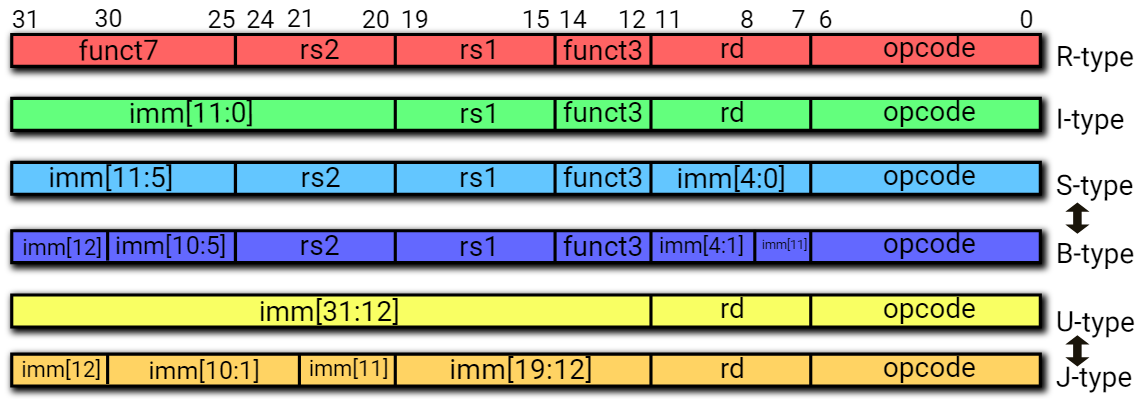
\includegraphics[width=1\textwidth]{CommandTypes}
			\caption{Instruction Types}
			\label{Image2.2}
		\end{center}
	\end{figure}
	\\

	The only difference between the S and B formats is that the 12-bit immediate field is used to encode branch offsets in multiples of 2 in the B format. Instead of shifting all bits in the instruction-encoded immediate left by one in hardware as is conventionally done, the middle bits (imm[10:1]) and sign bit stay in fixed positions, while the lowest bit in S format (inst[7]) encodes a high-order bit in B format.
	\\
	
	Similarly, the only difference between the U and J formats is that the 20-bit immediate is shifted left by 12 bits to form U immediates and by 1 bit to form J immediates. The location of instruction bits in the U and J format immediates is chosen to maximize overlap with the other formats and with each other.\\
	
	\begin{figure}[h!]
		
		\begin{center}
			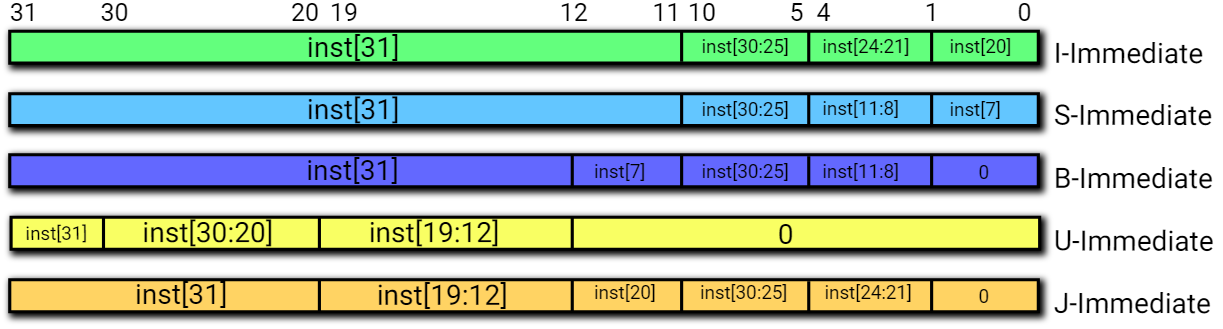
\includegraphics[width=1\textwidth]{ImmediateTypes}
			\caption{Immediate Types}
			\label{Image2.3}
		\end{center}
	\end{figure}

	The fields of Figure \ref{Image2.3} are labeled with the instruction bits (instr[y]) used to construct their value. Sign extension always uses inst[31]. \\
	
	Labeled as $rd$ is the destination register, meaning the register at which the result of the operation will be stored and as $rs1,rs2$ (if any) are the registers (operands) that will be used. The $funct7,funct3$ and $opcode$ fields will be used for the decode of the command and for the generation of the signals needed for its processing while the $imm[x:y]$ fields will be used for the assemble of the command's immediate.	
	\newpage
	\subsection{The Instructions}
	\label{subsec:ActualInstructions}
	\subsubsection{Integer Computational Instructions}
	\label{subsubsec:IntegerInstr}
	Most integer computational instructions operate on XLEN (= 32) bits of values held in the integer register file. Integer computational instructions are either encoded as register-immediate operations using the I-type format or as register-register operations using the R-type format. The destination is register $rd$ for both register-immediate and register-register instructions. \\
	Note that there is not a special instruction set support for overflow checks on integer arithmetic operations in the RV32I ISA. Overflow checks can be cheaply implemented using branches. \\
	The commands on the tables below follow the color-code of  Figure~\ref{Image2.2} and Figure~\ref{Image2.3} \\
	\vspace{4mm}
	\textbf{ {\footnotesize[A] Integer Register-Immediate Instructions }} \\
	
	\begin{threeparttable}
		\begin{tabular}{|c|p{3in}|p{1in}|} \hline
		\setrow{\bfseries}Command &\setrow{\bfseries} Operation &\setrow{\bfseries} Syntax 	\\\hline
		\cellcolor{brightgreen}ADDI & {\small Addition between $imm$ and $rs1$} & {\small $addi$ $rd,rs1,imm$} 	\\\hline
		\cellcolor{brightgreen}SLTI & {\small If $rs1<imm$ then $rd\leftarrow1$ else $rd\leftarrow0$} & {\small $slti$ $rd,rs1,imm$} \\\hline
		\cellcolor{brightgreen}SLTIU& {\small Same as SLTI, but UNSIGNED} &{\small $sltiu$ $rd,rs1,imm$} 			\\\hline
		\cellcolor{brightgreen}ANDI & {\small Bitwise AND between $rs1$ and $imm$} & {\small $andi$ $rd,rs1,imm$}	\\\hline
		\cellcolor{brightgreen}ORI  & {\small Bitwise OR between $rs1$ and $imm$} & {\small $ori$ $rd,rs1,imm$}   \\\hline
		\cellcolor{brightgreen}XORI & {\small Bitwise XOR between $rs1$ and $imm$} & {\small $xori$ $rd,rs1,imm$} \\\hline
		\cellcolor{brightgreen}SLLI & {\small Shift left logical of $rs1$ by given shift amount ($imm$)} & {\small $slli$ $rd,rs1,imm$} \\\hline
		\cellcolor{brightgreen}SRLI & {\small Shift right logical of $rs1$ by given shift amount($imm$)} &
		{\small $srli$ $rd,rs1,imm$} \\\hline
		\cellcolor{brightgreen}SRAI & {\footnotesize Shift right arithmetic of $rs1$ by given shift amount($imm$)} &
		{\small $srai$ $rd,rs1,imm$} \\\hline
		\cellcolor{canaryyellow}LUI &{\small $rd\leftarrow imm$} & {\small $lui$ $rd,imm$} \\\hline
		\cellcolor{canaryyellow}AUIPC&{\small $rd\leftarrow pc+imm$} & {\small $auipc$ $rd, imm$} \\\hline
			
		\end{tabular}

		 \begin{tablenotes}
		 	
			\footnotesize
			\item Notes:
			\item
			 \underline{\textbf{\textcolor{brightgreen}{$\rightarrow$}}} The arithmetic operations that include addition \underline{ignore} overflow scenarios as mentioned before. The immediates used in those commands are I-type Immediates and they are generated as shown at Figure~\ref{Image2.3}. Shifts by a constant are encoded as a specialization of the I-type format. The operand to be shifted is in $rs1$, and the shift amount is encoded in the lower 5 bits of the I-immediate field.
			\item 
			\underline{\textbf{\textcolor{canaryyellow}{$\rightarrow$}}} Those two instructions are of the U-type and use the respective Immediate types as well.  LUI stands for "Load Upper Immediate" while AUIPC stands for "Add Upper Immediate To PC". Again one can recur at Figure~\ref{Image2.3} for further details on the subject of Immediate generation.
			\captionof{table}{Register-Immediate Instructions}
			\label{subsubsec:table2.2}
			\vspace{4cm}
		\end{tablenotes}
	\end{threeparttable}
	
	\textbf{ {\footnotesize[B] Integer Register-Register Instructions }} \\
	
	\begin{threeparttable}
		\begin{tabular}{|c|p{3in}|p{1in}|} \hline
			\setrow{\bfseries}Command &\setrow{\bfseries} Operation &\setrow{\bfseries} Syntax 	\\\hline
			\cellcolor{bred}ADD & {\small Addition between $rs1$ and $rs2$} & {\small $add$ $rd,rs1,rs2$} 	\\\hline
			\cellcolor{bred}SUB & {\small Subtraction between $rs1$ and $rs2$} & {\small $sub$ $rd,rs1,rs2$}  \\\hline
			\cellcolor{bred}SLT & {\small If $rs1<rs2$ then $rd\leftarrow1$ else $rd\leftarrow0$} & {\small $slt$ $rd,rs1,rs2$} \\\hline
			\cellcolor{bred}SLTU & {\small Same as SLT, but UNSIGNED} &{\small $sltu$ $rd,rs1,rs2$} 			\\\hline
			\cellcolor{bred}AND  & {\small Bitwise AND between $rs1$ and $rs2$} & {\small $and$ $rd,rs1,rs2$} \\\hline
			\cellcolor{bred}OR   & {\small Bitwise OR between $rs1$ and $rs2$}  & {\small $or$ $rd,rs1,rs2$}  \\\hline
			\cellcolor{bred}XOR  & {\small Bitwise XOR between $rs1$ and $rs2$} & {\small $xor$ $rd,rs1,rs2$} \\\hline
			\cellcolor{bred} SLL & {\small Shift left logical of $rs1$ by given shift amount ($rs2$)}& {\small $sll$ $rd,rs1,rs2$} \\\hline
			\cellcolor{bred} SRL & {\small Shift right logical of $rs1$ by given shift amount ($rs2$)} & {\small $srl$ $rd,rs1,rs2$} \\\hline
			\cellcolor{bred} SRA & {\footnotesize Shift right arithmetic of $rs1$ by given shift amount ($rs2$)} & {\small $sra$ $rd,rs1,rs2$} \\\hline
			
		\end{tabular}
	
		 \begin{tablenotes}
			
			\footnotesize
			\item Notes:
			\item
			The shift amount is now held in the lower 5 bits of register $rs2$.
			\captionof{table}{Register-Register Instructions}
			\label{subsubsec:table2.3}
			\vspace{5mm}
		\end{tablenotes}

	\end{threeparttable}
	
	\textbf{ {\footnotesize[C] NOP Instruction }} \\
	
	The NOP instruction does not change any user-visible state, except for advancing the \textbf{pc}. NOP is encoded as $ADDI$ $x0,x0,0$. 
	\vspace{5mm}
	
	\subsubsection{Control Transfer Instructions}
	\label{subsubsec:ControlTransferInstr}
	
	The RV32I ISA provides two types of control transfer instructions: unconditional jumps and conditional branches. Control transfer instructions in RV32I do not have architecturally visible delay slots.\\
	
	\textbf{ {\footnotesize[A] Unconditional Jumps }} \\
	
	\begin{threeparttable}
		\begin{tabular}{|c|p{3in}|p{1in}|} \hline
			\setrow{\bfseries}Command &\setrow{\bfseries} Operation &\setrow{\bfseries} Syntax 	\\\hline
			\cellcolor{carorange}JAL & {\footnotesize $GOTO$ $pc+imm$ and $rd\leftarrow pc+4$} & $jal$ $rd,imm$ \\\hline
			\cellcolor{brightgreen}JALR & {\footnotesize $GOTO$ $(rs1+imm)[31:1]\&0$ and $rd\leftarrow pc+4$} & {\small$jalr$ $rd,rs1,imm$}\\\hline 
		\end{tabular}
		\begin{tablenotes}
		\footnotesize	
		\item 
		Notes:
		\item 
		\underline{\textbf{\textcolor{carorange}{$\rightarrow$}}} JAL (Jump and Link) is a J-type instruction. J-immediate encodes a signed offset in multiples of 2 bytes. The offset is sign-extended and added to the pc, to form the jump target address. Jumps can therefore target a $\pm1MiB range$. JAL stores the address of the instruction following the jump (pc+4) into register rd.
		\item 
		\underline{\textbf{\textcolor{brightgreen}{$\rightarrow$}}} JALR (Jump and Link Register) uses the I-type encoding. The jump target address is obtained by adding the 12-bit signed I-immediate to the register rs1, then setting the least-significant bit of the result to zero. The address of the instruction following the jump (pc+4) is written to register rd.
		\end{tablenotes}
		\captionof{table}{Uncoditional Jumps}
		\label{subsubsec:table2.4}
		\vspace{1cm}
	\end{threeparttable}

	\textbf{ {\footnotesize[B] Conditional Branches }} \\
	
	All branch instructions use the B-type instruction format. The 12-bit B-immediate encodes signed offsets in multiples of 2 and is added to the current pc to give the target address. The conditional branch range is $\pm4KiB$.\\
	
	\begin{threeparttable}
	
		\begin{tabular}{|c|p{3in}|p{1in}|} \hline
		\setrow{\bfseries}Command &\setrow{\bfseries} Operation &\setrow{\bfseries} Syntax 					 \\\hline
		\cellcolor{blue} BEQ & {\small $if$ $rs1=rs2$ then $JUMP$} & {\small $beq$ $rs1,rs2,imm$} 		 \\\hline
		\cellcolor{blue} BNE & {\small $if$ $rs1\neq rs2$ then $JUMP$} & {\small $bne$ $rs1,rs2,imm$} 	 \\\hline
		\cellcolor{blue} BLT & {\small $if$ $rs1<rs2$ then $JUMP$} & {\small $blt$ $rs1,rs2,imm$}		 \\\hline 
		\cellcolor{blue} BLTU & {\small Same as BLT, but UNSIGNED } & {\small $bltu$ $rs1,rs2,imm$}		 \\\hline
		\cellcolor{blue} BGE  & {\small $if$ $rs1\geq rs2$ then $JUMP$} & {\small $bge$ $rs1,rs2,imm$} 	 \\\hline
		\cellcolor{blue} BGEU & {\small Same as BGE, but UNSIGNED } & {\footnotesize $bgeu$ $rs1,rs2,imm$}\\\hline
		\end{tabular}
		
		\begin{tablenotes}
			\footnotesize
			\item 
			Notes:
			\item 
			The commands BGT, BGTU, BLE and BLEU can be synthesized by reversing the operands to BLT, BLTU, BGE and BGEU respectively.
			\captionof{table}{Conditional Branches}
			\label{subsubsec:table2.5}
			\vspace{5mm}
		\end{tablenotes}
		
	\end{threeparttable}
	
	\subsubsection{Load and Store Instructions}
	\label{subsubsec:LoadsStores}		
	
	
	RV32I is a load-store architecture, where only load and store instructions access memory and arithmetic instructions only operate on CPU registers. RV32I provides a 32-bit user address space that is byte-addressed and little-endian.
	The effective address in both cases is obtained by adding register $rs1$ to the sign-extended 12-bit offset.\vspace{3mm}
	
		\begin{threeparttable}
		
		\begin{tabular}{|c|p{3in}|p{1in}|} \hline
			
			\setrow{\bfseries}Command &\setrow{\bfseries} Operation &\setrow{\bfseries} Syntax 					 		 \\\hline
			\cellcolor{brightgreen} LW & {\small $rd\leftarrow MEM[31:0]$} & {\small $lw$ $rd,imm(rs1)$}		         \\\hline
			\cellcolor{brightgreen} LH & {\small $rd\leftarrow MEM[31:16]$ or $MEM[15:0]$} & {\small $lh$ $rd,imm(rs1)$} \\\hline
			\cellcolor{brightgreen} LHU &{\small Same as LH, but UNSIGNED} & {\small $lhu$ $rd,imm(rs1)$}                \\\hline
			\cellcolor{brightgreen} LB & {\footnotesize $rd\leftarrow MEM[31:24]$ or $MEM[23:16]$ or $MEM[15:8]$ or $MEM[7:0]$}
			& {\small $lb$ $rd,imm(rs1)$}                                                                                \\\hline
			\cellcolor{brightgreen} LBU &{\small Same as LB, but UNSIGNED} & {\small $lbu$ $rd,imm(rs1)$}                \\\hline
			\cellcolor{capri!75} SW & {\small $MEM\leftarrow rs2$} & {\small $sw$ $rs2,imm(rs1)$}                        \\\hline
			\cellcolor{capri!75} SH & {\small $MEM[31:16]$ or $MEM[15:0]$ $\leftarrow rs2[15:0]$} &{\small $sh$ $rs2,imm(rs1)$}                                                                                              \\\hline
			\cellcolor{capri!75} SB & {\footnotesize $MEM[31:24]$ or $MEM[23:16]$ or $MEM[15:8]$ or $MEM[7:0]$ $\leftarrow rs2[7:0]$}
			& {\small $sb$ $rs2,imm(rs1)$}                                                                               \\\hline
			
		\end{tabular}
		
		\begin{tablenotes}
			
			\footnotesize
			\item 
			Notes:
			\item 
			The choosing of the byte that will be written or loaded in any case is done by the 2 least-significant bits of the calculated effective address.
			\item
			\underline{\textbf{\textcolor{brightgreen}{$\rightarrow$}}} In case of LH/LB operations, the loaded value will be sign-extended up to 32-bits while in case of LHU/LBU, the value will be zero-filled up to 32-bits.
			\item 
			\underline{\textbf{\textcolor{capri!75}{$\rightarrow$}}} Always the least-significant bits of the register $rs2$ are being stored at SH and SB operations.
			
		\end{tablenotes}
	
		\captionof{table}{Loads and Stores}
		\label{subsubsec:table2.6}
		\vspace{5mm}
		
	\end{threeparttable}

	
	
%\end{document}
	\let\cleardoublepage\clearpage
	
	\definecolor{forestgreen(web)}{rgb}{0.13, 0.55, 0.13}
\definecolor{ao}{rgb}{0.0, 0.0, 1.0}
\definecolor{burgundy}{rgb}{0.5, 0.0, 0.13}
\definecolor{byzantium}{rgb}{0.44, 0.16, 0.39}
\chapter{Design of the RV32I Machine}
	\minitoc
	\vspace{5mm}
	In this chapter, as mentioned before, we will present one by one the CPU's pipeline stages and also the final design. Every part and every module that was created (via $VHDL$) was thoroughly tested before moving to the next one. The whole design consists of five pipeline stages which are the Instruction Fetch, the Instruction Decode, Execute Stage, Memory Stage and Write Back Stage. 
	\clearpage
	\section{Instruction Fetch - IF}
	 \label{Instruction Fetch}
	 The Instruction Fetch ($IF$) module consists of a simple memory block (M4K - block)\footnote{The use of M4K was mandatory in our case since we wanted the design to be synthesizable. Having that in mind, the only embedded memory available on our FPGA board was the M4K RAM memory type } that is used to simulate the Instruction Cache (I\$) in our system. 
	 We chose for the I\$ to have $1024$ slots which are $32$-bit wide (since we are implementing a 32-bit architecture). So the total capacitance of the memory is $4096$ B. 
	 
	 \begin{figure}[h!]
	 	\begin{center}
	 		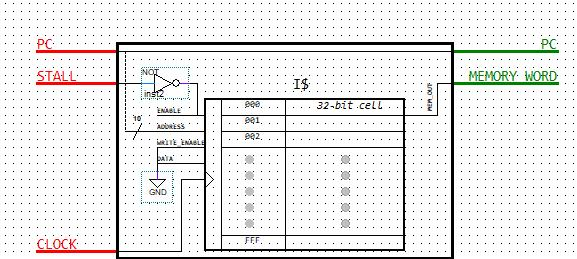
\includegraphics[width=1\textwidth]{IF}
	 		\caption{Instruction Fetch schematic}
	 		\label{Image3.1}
	 	\end{center}
	 \end{figure}
 
	 $IF$ is responsible for fetching the proper instruction ($MEMORY\_WORD$) from I\$. This is done by isolating some bits of the program counter ($PC$) and using them as address for the I\$. Since the memory has $1024$ slots we need $\log_2(1024)=\underline{10}$ bits to iterate through all of them and so, we use the $PC(11..2)$ bits for this work. \\
	 Module's I/O:	  
	
	 {\small
 	 \renewcommand{\labelenumii}{\Roman{enumii}}
	 \begin{itemize}
	 	\item Inputs:
	 	\begin{enumerate}
	 		
	 		\item \textcolor{red}{$CLOCK$} : System clock.
	 		\item \textcolor{red}{$STALL$} : Pipeline control signal (1-bit).
	 		\item \textcolor{red}{$PC$}    : Program counter (32-bit).
	 	\end{enumerate}
 		\item Outputs:
 		\begin{enumerate}
 		
 			\item \textcolor{forestgreen(web)}{$MEMORY\_WORD$} : Word fetched from I\$ (32-bit).
 			\item \textcolor{forestgreen(web)}{$PC$}	 	   : Program counter (32-bit).
 		\end{enumerate}
	 \end{itemize}}
 	\vspace{5mm}
 	 	
 	Last but not least the M4K Memory used was automatically generated by Quartus's II Mega-Wizard Plug-In Manager.
 	
 	\newpage
 	
 	\section{Instruction Decode - ID}
 	\label{Instruction Decode}
 	This is one of the most important and resourceful modules of this design. The Instruction Decode ($ID$) module is responsible for one thing among others; to "recognize" the command that was fetched on the previous cycle and activate all the signals that are needed for the command to be successfully processed.
 	
 		 \begin{figure}[h!]
 		\begin{center}
 			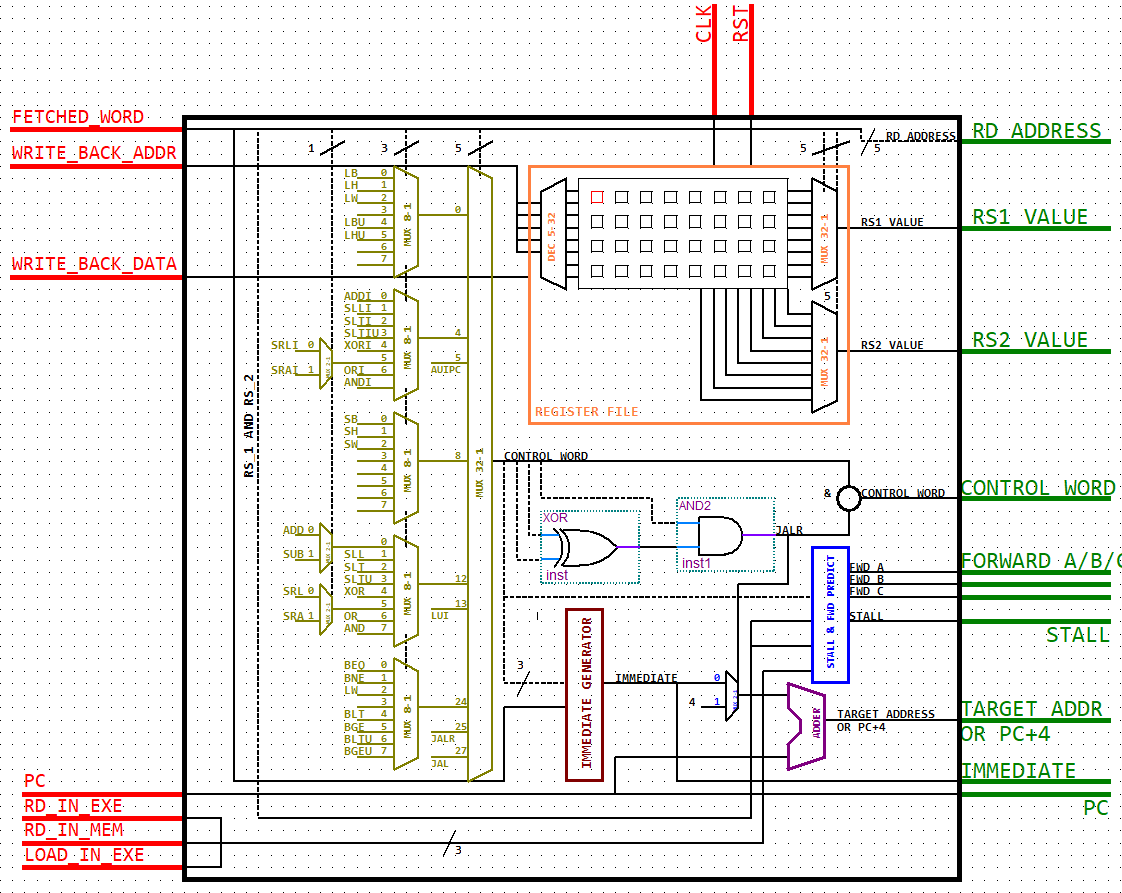
\includegraphics[width=1.0\textwidth]{DECODE}
 			\caption{Instruction Decode schematic}
 			\label{Image3.2}
 		\end{center}
 	\end{figure}
 	
 	\vspace{2mm}
 	
 	Designing the $ID$ module was a trial-and-error process due to the nature of the task that is asserted to it. While being the second part of the pipeline, its development suggests a deep knowledge of what will be done in one, two, and three clock cycles later for every(!) command that is currently being decoded. In this stage we also detect true dependencies ($RAWs$ %sto telos episis
 	) and handle them accordingly to maximize the performance when it is needed. Also, ID is being equipped with a simple \textcolor{byzantium}{Adder} so that it can calculate either the return address of a $JUMP$ or the target address ($PC+IMMEDIATE$) according to the Uncoditional Jump command that is currently being decoded. \\\\
 	Once again, we will follow the color-code of Figure \ref{Image3.2} so one can navigate through the design and the description.
 	
 	\clearpage
 	
 	\subsection{\textcolor{olive}{Multiplexer Network}}
 	\label{subsubsection3.2.1}
 	
 	Being tasked with the work of decoding the previously fetched instruction (\textbf{word}), we have to figure out a way to detect which one of the possible instructions it is. After the successful decode of the word, we have to provide all(!) the mandatory \textbf{control signals} for the next pipeline stages to make sure that all the necessary actions for the process of the now decoded instruction will be done.\\\\ At Section \ref{sect2.3.3} we listed all the instructions that belong to our $RV32I$ implementation. Also, Figure \ref{Image2.2} shows that all the instruction types have their 7 LSBs\footnote{Least Significant Bits} dedicated for the $opcode$ field. Also, in combination with Figure \ref{image2.1} we conclude that there is no point to process the two LSBs of any word that has to be decoded.\\\\
 	The first step for the process is to understand how the commands are being encoded by the Assembler; and to do so we used the official RISC-V Instruction Set Manual. The encoding of every command is displayed below at Table \ref{subsec3.2:table3.1}. Marked with bold style is all the information the Multiplexer Network uses to determine the identity of the command.
 	
 	Observing the encoding information displayed on Table \ref{subsec3.2:table3.1} we came to the following conclusions:
 	\begin{itemize}
 		\item According to their $opcode$ bits the commands are either stand-alone or belong in a group with other commands of similar type or functionality.
 		\item The groups are the following five:
 		\begin{itemize}
 			\item Loads
 			\item I-type arithmetics
 			\item Stores
 			\item R-type commands
 			\item Branches
 		\end{itemize}
 		\item Most of the commands that belong to a group, have a "unique" $funct3$ 3-bit code. 
 		\item Some of the grouped commands have the same $funct3$ code but have a different $funct7[5]$ bit.
 	\end{itemize}	
 	\vspace{2mm}
 	
 		 In conclusion the Multiplexer Network is responsible of selecting the correct control signal to pass to the following pipeline stages. Each multiplexer's input is a static control signal, which dictates what operations must be done in every stage for the successful process of the command. 
		
	\clearpage
	
 	\vspace{2mm}
 	\begin{threeparttable}[h!]
 		
	 	\begin{tabular}{|c|c|c|c|c|c|r|} \hline
	 	\multicolumn{4}{|c|}{imm[31:12]}	   &	rd	        & \textbf{01101}11                   & "LUI"                     \\\Xhline{5\arrayrulewidth}
	 	\multicolumn{4}{|c|}{imm[31:12]}	   &	rd	        &\textbf{00101}11                    & "AUIPC"                   \\\Xhline{5\arrayrulewidth}
	 	
	 	\multicolumn{4}{|c|}{imm[20\&10:1\&11\&19:12]}	& rd	&\textbf{11011}11 				     & "JAL" 				    \\\Xhline{5\arrayrulewidth}
	 	
	 	\multicolumn{2}{|c|}{imm[11:0] }       &	rs1	& 000	& rd  & \textbf{11001}11        	 & "JALR" 					\\\Xhline{5\arrayrulewidth}
	 	
	 	imm[12\&10:5] 						   & 	rs2	& rs1	& \setrow{\bfseries}000 & 	imm[4:1\&11]  	& \textbf{11000}11	& "BEQ" 		\\\hline
	 	imm[12\&10:5] 						   & 	rs2	& rs1	& \setrow{\bfseries}001 & 	imm[4:1\&11] 	& \textbf{11000}11	& "BNE" 		\\\hline
	 	imm[12\&10:5] 						   & 	rs2	& rs1	& \setrow{\bfseries}100 & 	imm[4:1\&11] 	& \textbf{11000}11	& "BLT" 		\\\hline
	 	imm[12\&10:5] 						   & 	rs2	& rs1	&\setrow{\bfseries} 101 & 	imm[4:1\&11] 	& \textbf{11000}11	& "BGE" 		\\\hline
	 	imm[12\&10:5] 						   & 	rs2	& rs1	& \setrow{\bfseries}110 & 	imm[4:1\&11] 	& \textbf{11000}11	& "BLTU" 		\\\hline
	 	imm[12\&10:5] 						   & 	rs2	& rs1	&\setrow{\bfseries} 111 & 	imm[4:1\&11] 	& \textbf{11000}11	& "BGEU" 		\\\Xhline{5\arrayrulewidth}
	 	
	 	\multicolumn{2}{|c|}{imm[11:0]}        &   rs1 & \setrow{\bfseries}000   & rd & \textbf{00000}11 & "LB"  \\\hline
	 	\multicolumn{2}{|c|}{imm[11:0]}		   &   rs1 & \setrow{\bfseries}001   & rd & \textbf{00000}11 & "LW"  \\\hline
	 	\multicolumn{2}{|c|}{imm[11:0]}        &   rs1 & \setrow{\bfseries}010   & rd & \textbf{00000}11 & "LW"  \\\hline
	 	\multicolumn{2}{|c|}{imm[11:0]}  	   & 	rs1 & \setrow{\bfseries}100  & rd & \textbf{00000}11 & "LBU" \\\hline
	 	\multicolumn{2}{|c|}{imm[11:0]} 	   &   rs1 & \setrow{\bfseries}101   & rd & \textbf{00000}11 & "LHU" \\\Xhline{5\arrayrulewidth}
	 	
	 	imm[11:5] & rs2 & rs1 & \setrow{\bfseries}000 & imm[4:0] & \textbf{01000}11 & "SB" \\\hline
	 	imm[11:5] & rs2 & rs1 & \setrow{\bfseries}001 & imm[4:0] & \textbf{01000}11 & "SH" \\\hline
	 	imm[11:5] & rs2 & rs1 & \setrow{\bfseries}010 & imm[4:0] & \textbf{01000}11 & "SW" \\\Xhline{5\arrayrulewidth}
	 	
		\multicolumn{2}{|c|}{imm[11:0]} & rs1 & \setrow{\bfseries}000 & rd &\textbf{00100}11 & "ADDI"  \\\hline
		\multicolumn{2}{|c|}{imm[11:0]} & rs1 & \setrow{\bfseries}010 & rd &\textbf{00100}11 & "SLTI"  \\\hline
		\multicolumn{2}{|c|}{imm[11:0]} & rs1 & \setrow{\bfseries}011 & rd &\textbf{00100}11 & "SLTIU" \\\hline
		\multicolumn{2}{|c|}{imm[11:0]} & rs1 & \setrow{\bfseries}100 & rd &\textbf{00100}11 & "XORI"  \\\hline
		\multicolumn{2}{|c|}{imm[11:0]} & rs1 & \setrow{\bfseries}110 & rd &\textbf{00100}11 & "ORI"   \\\hline
		\multicolumn{2}{|c|}{imm[11:0]} & rs1 & \setrow{\bfseries}111 & rd &\textbf{00100}11 & "ANDI"  \\\hline
		0000000 & shamt & rs1 & \setrow{\bfseries}001 & rd &\textbf{00100}11 & "SLLI" \\\hline
		0000000 & shamt & rs1 & \setrow{\bfseries}101 & rd &\textbf{00100}11 & "SRLI" \\\hline
		0\textbf{1}00000 & shamt & rs1 & \setrow{\bfseries}101 & rd & \textbf{00100}11 & "SRAI" \\\Xhline{5\arrayrulewidth}
		
		0000000 & rs2   & rs1 & \setrow{\bfseries}000 & rd & \textbf{01100}11 & "ADD"  \\\hline
		0\textbf{1}00000 & rs2   & rs1 & \setrow{\bfseries}000 & rd & \textbf{01100}11 & "SUB"  \\\hline
		0000000 & rs2   & rs1 & \setrow{\bfseries}001 & rd & \textbf{01100}11 & "SLL"  \\\hline
		0000000 & rs2   & rs1 & \setrow{\bfseries}010 & rd & \textbf{01100}11 & "SLT"  \\\hline
		0000000 & rs2   & rs1 & \setrow{\bfseries}011 & rd & \textbf{01100}11 & "SLTU" \\\hline
		0000000 & rs2   & rs1 & \setrow{\bfseries}100 & rd & \textbf{01100}11 & "XOR"  \\\hline
		0000000 & rs2   & rs1 & \setrow{\bfseries}101 & rd & \textbf{01100}11 & "SRL"  \\\hline
		0\textbf{1}00000 & rs2   & rs1 & \setrow{\bfseries}101 & rd & \textbf{01100}11 & "SRA"  \\\hline
		0000000 & rs2   & rs1 & \setrow{\bfseries}110 & rd & \textbf{01100}11 & "OR"   \\\hline
		0000000 & rs2   & rs1 & \setrow{\bfseries}111 & rd & \textbf{01100}11 & "AND"  \\\hline
	 	\end{tabular}
 		
 		\begin{tablenotes}
 		\footnotesize
 		\item 
 		Notes:
 		\item 	
 		"\&" is the concatenation operator.
 		\end{tablenotes}
 		
 		\captionof{table}{RV32I Command Encoding}
 		\label{subsec3.2:table3.1}
 		\vspace{5mm}
 		
 	\end{threeparttable}
 
 	\clearpage
	 	 
	 Starting from right to left, there is a $32\rightarrow1$ multiplexer. This multiplexer is used to select the correct group of the command (if the command belongs to a group) or the stand-alone command itself(e.g. "AUIPC"). This is done by using the $opcode[6..2]$ bits of the word as selector. Since the $opcode[6..2]$ bits alter from command to command in a non-sequential manner, we use all five of them and end up with a $2^{5}=32\rightarrow1$ multiplexer.\\
	 
	 Following behind, there are five $8\rightarrow1$ multiplexers which use the three $funct3$ bits (if any) of the word to select a specific command inside a group. Note that since we have five different command groups, we use five multiplexers in this layer.\\
	 
	 Some of the commands, belong to the same group and also have the same $funct3$ code (e.g. "ADD" - "SUB"). To separate them we utilize the $funct7[5]$ bit of the word which changes in that case. So, using this bit as selector we attach to the network three $2\rightarrow1$ multiplexers and so, we cover all the possible scenarios of decoding.\\
	 
	
	\subsubsection{Multiplexer Input}
	\label{subsub:muxin}
	
	As mentioned above, the input of every multiplexer is a static, hard-typed control signal of $20$ bits of the following format. \\
	
	\begin{figure}[h!]
		\begin{center}
			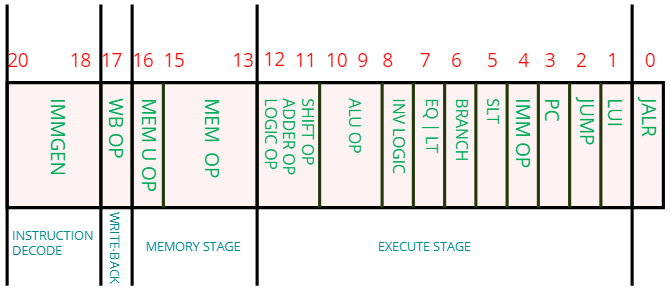
\includegraphics[width=0.7\textwidth]{ControlWord}
			\caption{Control Word Format}
			\label{Image3.3}
		\end{center}
	\end{figure}	

	\vspace{2mm}
	
	Depicted with blue color at Figure \ref{Image3.3} are four groups of bits. These are the bits that concern each pipeline stage. The bit $0$ is used also at ID stage along with bits $20..18$ but it is appended later as Figure \ref{Image3.2} shows and is not hard-type in every input of the multiplexers like the rest of the control signal bits. It is also used for pipeline control.
	
	\clearpage
	\small
	\begin{itemize}
		%\setlength\itemsep{-0.1em}
		\item \textbf{IMMGEN} : Immediate Genaration
		\begin{itemize}
			\setlength\itemsep{-0.1em}
			\item $000$ : I-type Immediate,
			\item $001$ : S-type Immediate.
			\item $010$ : B-type Immediate.
			\item $011$ : U-type Immediate.
			\item $100$ : J-type Immediate.
		\end{itemize}
		\item \textbf{WB OP} : Write Back operation. $0$ if the command doesn't require a Write Back action, $1$ if it does.
		\item \textbf{MEM U OP} : Memory Unsigned Operation. $0\rightarrow NO$, $1\rightarrow YES$.
		\item \textbf{MEM OP} : Memory Operation.
		\begin{itemize}
			\setlength\itemsep{-0.1em}
			\item $000$ : LB 
			\item $001$ : LH
			\item $010$ : LW
			\item $100$ : SB
			\item $101$ : SH
			\item $110$ : SW
			\item $111$ : MEM-Free operation.
		\end{itemize}
		\item \textbf{ALU OP}: ALU Operation 
		\begin{itemize}
			\setlength\itemsep{-0.1em}
			\item $00$ : Addition.
			\item $01$ : Subtraction.
			\item $10$ : Logic Operation.
			\item $11$ : Shift Operation.
		\end{itemize}
		\item \textbf{SHIFT/ADDER/LOGIC OP}: Since bits $[9..8]$ determine which ALU module will be used there is no problem using the same bits $[11..10]$ to represent different operations in different ALU modules. 
		\begin{itemize}
			\setlength\itemsep{-0.3em}
			\item Shift Module:
			\begin{itemize}
				\setlength\itemsep{-0.1em}
				\item $00$ : Shift Right Logical.
				\item $01$ : Shift Left Logical.
				\item $10$ : Shift Right Arithmetic.
			\end{itemize}
			\item Adder Module:
			\begin{itemize}
				\setlength\itemsep{-0.1em}				
				\item $0X$ : Signed Addition or Subtraction.
				\item $1X$ : Unsigned Addition or Subtraction.

			\end{itemize}
			\item Logic Module:
			\begin{itemize}
				\setlength\itemsep{-0.1em}
				\item $00$ : And.
				\item $01$ : Or.
				\item $10$ : Xor.			
			\end{itemize}
		\end{itemize}
		
		\item \textbf{INV}\textbf{ \& EQ/LT}: Used for resolving a branch case. 
		\item \textbf{BRANCH}: $0\rightarrow$ the command is not a Branch, $1\rightarrow$ the command is a Branch.
		\item \textbf{SLT}: $0\rightarrow$ the command is not SLT, $1\rightarrow$ the command is SLT.
		\item \textbf{PC}: $0\rightarrow$ PC is not required for calculations. $1\rightarrow$ PC is required for calculations.
		\item \textbf{JUMP}: $0\rightarrow$ the command is not a JUMP. $1\rightarrow$ command is a JUMP.
		\item \textbf{LUI}: $0\rightarrow$ the command is not a LUI. $1\rightarrow$ the command is a LUI.
		\item \textbf{JALR}: $0\rightarrow$ the command is not a JALR. $1\rightarrow$ the command is a JALR.
	\end{itemize}
	
	\clearpage
		
	\begin{center}
		\begin{threeparttable}[!ht]
			\begin{tabular}{|c|c|} \hline
				
				\setrow{\bfseries}Command &\setrow{\bfseries} Control-Word \\\hline
				LB   &000-1-0-000-0X-00-X-X-0-0-1-0-0-0-0 \\\hline
				LH   &000-1-0-001-0X-00-X-X-0-0-1-0-0-0-0\\\hline
				LW   &000-1-0-010-0X-00-X-X-0-0-1-0-0-0-0\\\hline
				LBU  &000-1-1-000-0X-00-X-X-0-0-1-0-0-0-0\\\hline
				LHU  &000-1-1-001-00-00-X-X-0-0-1-0-0-0-0\\\Xhline{5\arrayrulewidth}
				
				ADDI &000-1-X-111-0X-00-X-X-0-0-1-0-0-0-0\\\hline
				SLLI &000-1-X-111-01-11-X-X-0-0-1-0-0-0-0\\\hline
				SLTI &000-1-X-111-0X-01-X-X-0-1-1-0-0-0-0\\\hline 
				SLTIU&000-1-X-111-1X-01-X-X-0-1-1-0-0-0-0\\\hline 
				XORI &000-1-X-111-10-10-X-X-0-0-1-0-0-0-0\\\hline 
				SRLI &000-1-X-111-00-11-X-X-0-0-1-0-0-0-0\\\hline
				SRAI &000-1-X-111-10-11-X-X-0-0-1-0-0-0-0\\\hline
				ORI  &000-1-X-111-01-10-X-X-0-0-1-0-0-0-0\\\hline
				ANDI &000-1-X-111-00-10-X-X-0-0-1-0-0-0-0\\\Xhline{5\arrayrulewidth}
				
				SB &001-0-0-100-0X-00-X-X-0-0-1-0-0-0-0\\\hline
				SH &001-0-0-101-0X-00-X-X-0-0-1-0-0-0-0\\\hline
				SW &001-0-0-110-0X-00-X-X-0-0-1-0-0-0-0\\\Xhline{5\arrayrulewidth}
				
				ADD &XXX-1-X-111-0X-00-0-0-0-0-0-0-0-0-0\\\hline
				SUB &XXX-1-X-111-0X-01-0-0-0-0-0-0-0-0-0\\\hline
				SLL &XXX-1-X-111-01-11-0-0-0-0-0-0-0-0-0\\\hline
				SLT &XXX-1-X-111-0X-01-0-0-0-1-0-0-0-0-0\\\hline
				SLTU&XXX-1-X-111-1X-01-0-0-0-1-0-0-0-0-0\\\hline
				XOR &XXX-1-X-111-10-10-0-0-0-0-0-0-0-0-0\\\hline
				SRL &XXX-1-X-111-00-11-0-0-0-0-0-0-0-0-0\\\hline
				SRA &XXX-1-X-111-10-11-0-0-0-0-0-0-0-0-0\\\hline
				OR  &XXX-1-X-111-01-10-0-0-0-0-0-0-0-0-0\\\hline
				AND &XXX-1-X-111-00-10-0-0-0-0-0-0-0-0-0\\\Xhline{5\arrayrulewidth}
				
				BEQ &010-0-X-111-0X-01-0-1-1-0-0-0-0-0-0\\\hline
				BNE &010-0-X-111-0X-01-1-1-1-0-0-0-0-0-0\\\hline
				BLT &010-0-X-111-0X-01-0-0-1-0-0-0-0-0-0\\\hline
				BGE &010-0-X-111-0X-01-1-0-1-0-0-0-0-0-0\\\hline
				BLTU&010-0-X-111-1X-01-0-0-1-0-0-0-0-0-0\\\hline
				BGEU&010-0-X-111-1X-01-1-0-1-0-0-0-0-0-0\\\Xhline{5\arrayrulewidth}
				
				AUIPC&011-1-X-111-0X-00-X-X-0-0-1-1-0-0-0\\\hline
				LUI  &011-1-X-111-XX-00-X-X-0-0-1-1-0-1-0\\\hline
				JALR &000-1-X-111-01-00-X-X-0-0-1-0-1-0-1\\\hline
				JAL  &100-1-X-111-0X-00-X-X-0-0-1-1-1-0-0\\\Xhline{5\arrayrulewidth}
										
			\end{tabular}
				\begin{tablenotes}
				\footnotesize
				\item 
				Notes:
				\item 	
				"X" stands for "Don't Care". It could be either 1 or 0.
				\end{tablenotes}
				
			 	\captionof{table}{Commands and their Control-Words}
				\label{subsec3.2:table3.2}
				\vspace{3mm}
		\end{threeparttable}
	
\end{center}

	This encoding, is the result of many iterations due to the fact that while being in the second pipeline stage ($ID$) we had to think about what will be needed to be done in the next pipeline stages. Finally, with respect to the encoding, we present the control-words (multiplexer inputs) for every instruction in our ISA.\\

\subsection{\textcolor{orange}{Register File}}

	The register file consists of $32$ registers which are $32$-bit wide as our architecture dictates. They all have the function of \textbf{read} and \textbf{write}(parallel load) except for one, the register $0$ which has the value $0$ hardwired inside it. This value cannot be altered meaning the register cannot do a parallel load operation. All other registers have a $RESET$ and a $LOAD$ control signal also which are activated only when a global\footnote{When the CPU starts running, we assume that there will be a short reset to initialize all the pipeline components} reset happens.\\
	
	As shown in Figure \ref{Image3.2} the register file is between a $5\rightarrow32$ decoder and two $32\rightarrow1$ multiplexers.
	The decoder is used for the $WRITE$ operations and the multiplexers are used for the $READ$ operations. Almost every command in our ISA has $5$ bits ($[11..7]$)\footnotemark dedicated for the register $rd$ which is the destination register, meaning the register in whom the result of the command will be written into. In our pipeline architecture this happens at the fifth (Write Back) stage. So, when a command reaches the Write Back stage and if it is a command that has to write a result into a register, then the Write Back provides the $rd$'s address back to the register file along with the value that has to be written (operation's result). The $rd$'s address is connected to the decoder and then the proper $LOAD$ signal is activated so that the register that translates to $rd$'s address will be ready for a $WRITE$ operation.\\
	
	The two multiplexers, are used to provide the operands, $rs1$ and $rs2$ (if any) values for the Execute Stage. They first multiplexer provides the $rs1$ value by using the word's bits$[19..15]$\footnotemark[\value{footnote}]. as selector while the second multiplexer provides the $rs2$ value by using the word's bit$[24..20]$\footnotemark[\value{footnote}]. as selector. Every multiplexer input is paired with every register's output. For example, $Reg_0\rightarrow I_0$, $Reg_1 \rightarrow I_1$, $Reg_2 \rightarrow I_2$ etc. \\
	
	Of course, not every command requires a $rs1$ or $rs2$ value. In this case the register file will provide two values that will be random and that will not be needed. Later, we add further logic components to resolve this issue. 
	
	
	\footnotetext{You can refer to Figure \ref{Image2.2} for any clarifications needed.}
\subsection{\textcolor{burgundy}{Immediate Generator}}
\label{subsection3.3}
The Immediate Genarator module is responsible for providining the immediate that is required according to the instruction that is being decoded. It uses the three bits$[20..18]$of the control word(Figure \ref{Image3.3})  and according to them, formats the proper immediate as Figure \ref{Image2.3} shows; by rearranging and manipulating the bits of the fetched word. When this procedure is over, the bits$[20.18]$ of the control word are no longer needed and thus they are removed of the control-word, before it leaves the $ID$ stage. \\

The behavioral architecture of the Immediate Generator module implements the following algorithm:
	
\begin{algorithm}[H]
	\SetAlgoLined
	\SetKwInOut{Input}{input}\SetKwInOut{Output}{output}
	
	\Input{ $CONTROL\_WORD[20..18]$ and $FETCHED\_WORD$}
	\Output{$IMMEDIATE$} 
	\BlankLine
	
	\emph{IMM\_TYPE $\leftarrow$ CONTROL\_WORD[20..18]}\;
	\uIf	{IMM\_TYPE == "000"} { {\small $IMMEDIATE$ =  \underline{I-type} Immediate, f(\footnotesize{$FETCHED\_WORD$})} \;}
	\uElseIf{IMM\_TYPE == "001"} { {\small $IMMEDIATE$ =  \underline{S-type} Immediate, f(\footnotesize{$FETCHED\_WORD$})} \;}
	\uElseIf{IMM\_TYPE == "010"} { {\small $IMMEDIATE$ =  \underline{B-type} Immediate, f(\footnotesize{$FETCHED\_WORD$})} \;}
	\uElseIf{IMM\_TYPE == "011"} { {\small $IMMEDIATE$ =  \underline{U-type} Immediate, f(\footnotesize{$FETCHED\_WORD$})} \;}
	\uElseIf{IMM\_TYPE == "100"} { {\small $IMMEDIATE$ =  \underline{J-type} Immediate, f(\footnotesize{$FETCHED\_WORD$})} \;}
	\Else{ {\small $IMMEDIATE$ =  \underline{XXX..X}} \;}
	
	\caption{Immediate Generator Algorithm}
\end{algorithm}	
\vspace{5mm}

\subsection{\textcolor{byzantium}{Adder}}
\label{subsection3.4}

In the the case of Uncoditional Jumps, two calculations are required. The calculation of the target address, and the storing of the next instruction's address, the return address,($PC+4$) to register rd. This translates into two addition operations that must be done in the event of those commands. All the computational force in a pipeline usually is entrusted to the pipeline's ALU\footnote{Arithmetic and Logic Unit}. In our pipeline ALU lays in the third stage, the $Execute$ stage. So we would have to equip the ALU module with two Adders since when a jump is imminent, two additions should be done. To relieve some workload of the ALU's design we decided to equip the $ID$ module with one of those two adders, an adder that will be responsible only for the calculation of the target address of the unconditional jumps. \\

In theory, this would work fine, since all the necessary operands are available at $ID$ stage. After further investigating the $JALR$ command though, we see that the target address is calculated in a different way. Instead of $PC+IMM$, $JALR$ dictates that the target address is calculated as $PC+RS1$. So this means that first, we have to access the register file to acquire the one of the two operands and then do the addition operation, since the $PC$ value is already available (from the $IF$ stage). In practice, we found that due to some propagation delays we should handle the $JALR$ case differently. \\ 
\clearpage
What we did to resolve this, is to treat the $JAL$ and $JALR$ commands in $ID$ like this:

\begin{itemize}
	\setlength\itemsep{-0.1em}
	\item If the command is $JAL$ then:
		\begin{itemize}
			\item Calculate the $TARGET\_ADDRESS$ as $PC+IMMEDIATE$.
		\end{itemize}
	\item If the command is $JALR$ then:
		\begin{itemize}
			\item Calculate the $RETURN\_ADRESS$ as $PC+4$.
		\end{itemize}
\end{itemize}

\vspace{2mm}

This is achieved by adding a $2\rightarrow1$ multiplexer that selects by $CONTROL\_WORD[0]$ - ($JALR$) either the $IMMEDIATE$ or the constant $+4$. So for $JAL$ we leave the calculation of the jump's return address to the $Execute$ stage and for $JALR$ we leave the calculation of the jump's target address to the $Execute$ stage.

\subsection{\textcolor{ao}{Stall \& Forward Predictor}}

This is a module that was added later on $ID$ and it is responsible for detecting whether a stall or a forwarding is required. Forwarding (or Bypassing) is the counter-measure of the true dependency RAW\footnote{Read After Write}, which is the only threat in our system, since we do not support OOO\footnote{Out Of Order execution}.

\begin{figure}[h!]
	\begin{center}
		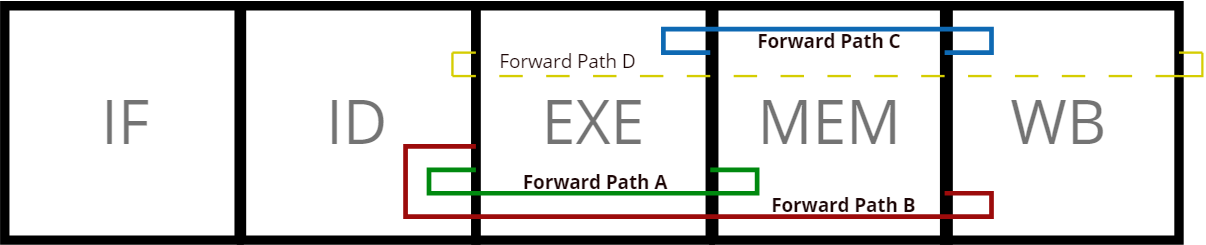
\includegraphics[width=1\textwidth]{FORWARDS}
		\caption{Forwarding Paths}
		\label{Image3.4}
	\end{center}
\end{figure}
\vspace{2mm}

The module is responsible for handling Forwards A,B, and C, while forward D\footnote{We will analyze the Forward D later.} is being handled by some external logic. So there are three main RAW scenarios that require resolution.

\subsubsection{Scenario A} 
\label{3.2.5.1}

\begin{lstlisting}[caption={Forward Path A Example},captionpos=b]
	OP_A	Reg_X, Reg_A, Reg_B
	OP_B 	Reg_Y, Reg_X, Reg_C
\end{lstlisting}



This scenario concerns the $ID$ and $Execute$ stages. OP\_A writes its result to Reg\_X. Then OP\_B requires Reg\_X's value as $rs1$ operand. Without the forwarding path, we would have to stall for at least two clock cycles and wait for OP\_A to reach the $Write\ Back$ stage. We know that the value that will be written at at Reg\_X will be available at the end of $Execute$ stage. So instead of stalling for two clock cycles, we activate the Forward Path A and transfer the value needed to OP\_B.

\clearpage

\subsubsection{Scenario B}
\label{3.2.5.2}

\begin{lstlisting}[caption={Forward Path B Example},captionpos=b]
	OP_A	Reg_X, Reg_A, Reg_B
	....	.....  .....  .....
	OP_B 	Reg_Y, Reg_X, Reg_C
\end{lstlisting}

This scenario concerns the $ID$ and $Memory$ stages. Once again OP\_A writes its result to Reg\_X and then, after one command that is in-between them, OP\_B requires this value as an operand. If not for the Forward Path B, we would have to stall again for one clock cycle and wait for OP\_A to reach the $Write\ Back$ stage.

\subsubsection{Scenario C}

\begin{lstlisting}[caption={Forward Path C Example},captionpos=b]
	LOAD 	Reg_X, IMM(Reg_A)
	STORE	Reg_X, IMM(Reg_B)
\end{lstlisting}

This scenario concerns only the $Memory$ stage. It only occurs when there is a $STORE$ command after a $LOAD$ command, of whom the later wishes to write in the memory the register value that the first has loaded. We would normally have to stall for one clock cycle again but with the Forward Path C we can overcome this issue. 

\subsubsection{Stall Generation}
\begin{lstlisting}[caption={Stall Scenario},captionpos=b]
LOAD 	Reg_X, IMM(Reg_A)
OP_A	Reg_A, Reg_X, Reg_B
\end{lstlisting}

In this case, we have to stall the OP\_A and those who follow, because the $LOAD$ command, has to reach the $Memory$ stage and then, activate the Forward Path B so that it can provide the needed value. This happens due to the nature of the $LOAD$ commands, which have their result ready at the end of $Memory$ stage and not at the $Execute$ stage like the other computational commands.\\

Here, we present an algorithm that represents the Stall \& Forward Predictor module's behavior. 

\begin{algorithm}[H]
	\SetAlgoLined
	\SetKwInOut{Input}{input}\SetKwInOut{Output}{output}
	
	\Input{ $RS1[4..0]$,$RS2[4..0]$, $RD\_IN\_EXE[4..0]$, $RD\_IN\_MEMORY[4..0]$, $LOAD\_IN\_EXE$, $CONTROL_WORD[20..18]$}
	\Output{ $FWDA$, $FWDB$, $FWDC$, $STALL$} 
	\BlankLine
	\BlankLine
	
	\emph{{\small $COMMAND\_IN\_ID \leftarrow f({\scriptsize CONTROL\_WORD[20..18]})$} {\footnotesize= (R/S/U/B/J)}} \;
	\BlankLine
	\If{$RS1$ == $RD\_IN\_EXE$ AND \underline{$RS1\neq REG_{0}$}} { \small $FWD\_A\_RS1 \leftarrow 1$\;}
	
	\If{$RS2$ == $RD\_IN\_EXE$ AND \underline{$RS2\neq REG_{0}$}} { \small $FWD\_A\_RS2 \leftarrow 1$\;}
	
	
	\If{IMM\_TYPE == "010"} { {\small $IMMEDIATE$ =  \underline{B-type} Immediate, f(\footnotesize{$FETCHED\_WORD$})} \;}
	\uElseIf{IMM\_TYPE == "011"} { {\small $IMMEDIATE$ =  \underline{U-type} Immediate, f(\footnotesize{$FETCHED\_WORD$})} \;}
	\uElseIf{IMM\_TYPE == "100"} { {\small $IMMEDIATE$ =  \underline{J-type} Immediate, f(\footnotesize{$FETCHED\_WORD$})} \;}
	\Else{ {\small $IMMEDIATE$ =  \underline{XXX..X}} \;}
	
	\caption{Stall and Forward Predictor Algorithm}
\end{algorithm}	

	\let\cleardoublepage\clearpage
	
	\chapter{Evaluation of the RV32I Machine}
\label{Chapter4}

\minitoc

\section{Exploring The Official Tests}
\label{Sec4.1:TESTS}

Since we completed the design of our system its now time to test it so that we can be sure that our work is accurate. To do so, we searched at the official  \href{https://github.com/riscv}{RISC-V GitHub repository} and we found out that they actually provide a toolchain in which, various tests for every architecture can be found. So after installing and configuring their software, we retrieved 37 $.s$ files which were later broke down to .hex and .dump files. So for every instruction in our ISA we have one $.dump$ file and one $.hex$ file. \\

The official RV32I tests have the following structure:
\begin{itemize}
	\setlength\itemsep{-0.1em}
	\item Every test file (for every instruction) has many mini-tests inside it. 
	\item Every mini-test:
		\vspace{-2mm}
		\begin{itemize}
			\setlength\itemsep{-0.1em}
			\item Uses the instruction in which it is dedicated.
			\item On success it updates the $GP$\footnote{Global Pointer} register and moves to the next one.
			\item On failure it jumps to an $ECALL$ instruction which has a specific opcode and terminates the test \footnote{Since the $ECALL$ command is not included to our current ISA, for the purpose of testing we added one extra signal to the $ID$ module which is the $ECALL$ signal. When it comes it simply the signal takes the value 1 and so we understand that the test is finished} .
		\end{itemize}
\end{itemize}

Judging by the way the tests were programmed we conclude that they were designed so that they can guarantee that every possible hazardous scenario for every instruction has been accounted for and avoided. We will mention some cases which we haven't initially considered but we discovered later during testing the pipeline. Alternatively we could try and use our own tests but unfortunately we could not find a stand-alone assembler for our cause. This means that in order to test the system ourselves we would have to program our very own RV32I Assembler...\\
\vspace{-6mm}
\section{Testing Procedure}
\label{Sec4.2:TESTING}
After understanding the testing logic, we used python (version 3) to create a script that takes the $.hex$ file and generates a $.mif$\footnote{Memory Initialization File} which represents the loaded I\$. For $LOADS$ and $STORES$ which had some values stored in D\$ we manually initialized the data cache $.mif$ files for every test. In conclusion we end up with 37 different $.mif$ files for I\$ and also 8 $.mif$ files for D\$ \footnote{There are 5 tests for all the $LOAD$ instructions and 3 for all $STORE$ instructions.}. All that's left now is to run one timing simulation for every test that we have. For our initial tests we used Quartus-II \footnote{Version 9.1sp Web Edition} embedded simulator. Unfortunately the first tests were not successful (as we expected) due to various logic errors in the final structural design and the debug process was not easy because we could not probe the suspicious internal nodes and signals easily using this simulator. We had to modify every file and add extra signals so that they could show up at the simulation. This means alternation to package files and all modules that use the circuit in which we appended a new probing signal to observe. \\

After many debug attempts, we switched to ModelSim where we could easily add and remove every node we wished in the simulation window, something that we made our debug process much easier than it was before. So after various errors we spotted during the testing process we were able to finally find and fix every bug that we found. But for every change we made we couldn't be sure that this change, would not affect previous tests that were completed successfully. So after the final/last changes we made we performed a regression testing, meaning that we run all the tests again. The results were satisfying, since every test was completed successfully. 
\vspace{-4mm}
\subsection{A Test Example}
\label{SubSec4.2.1:EXAMPLE}

We will now showcase a sample of our testing process. This test concerns the "ADDI" command. All we need is just the $.dump$ file so that we can understand and follow the simulation and also we need the simulation window. The "ADDI" test file has 25 mini-tests so we cannot go through all of them. We will present the first of those tests and its prosperous results. 

\begin{figure}[h!]
	\begin{center}
		\fbox{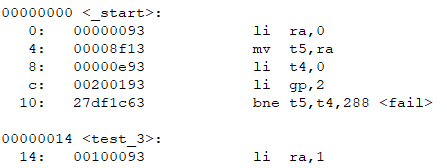
\includegraphics[width=0.7\textwidth]{ADDITEST2}}
		\caption{ADDI test \#2.}
		\label{Image4.1}
	\end{center}
\end{figure}

\clearpage

\begin{figure}[h!]
	\begin{center}
		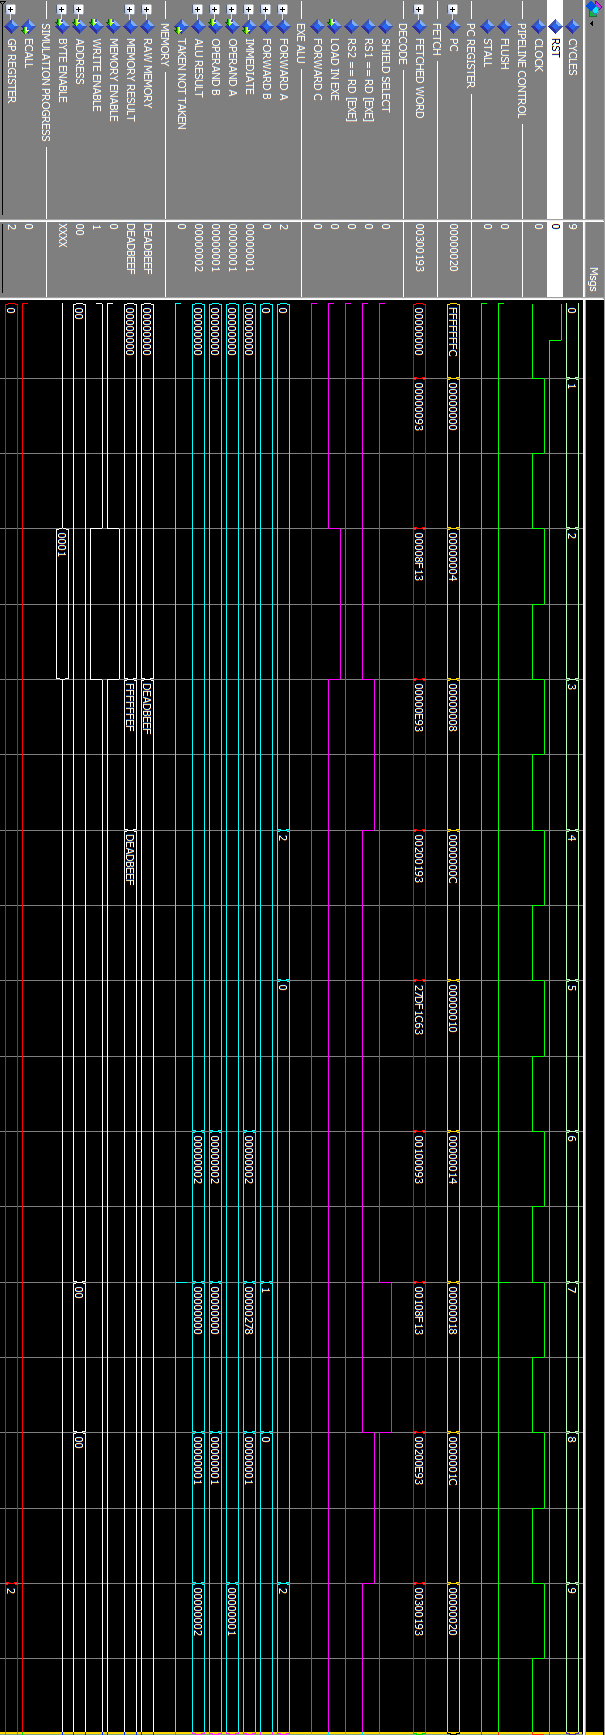
\includegraphics[height = 0.9\textheight,width=1\textwidth]{MODELSIM}
		\caption{ModelSim simulation of the "ADDI" test \#2.}
		\label{Image4.2}
	\end{center}
\end{figure}

\clearpage
\subsubsection{About the Figure \ref{Image4.1}}
The Load Immediate ($li$) command is a pseudo-operation which translates to: $addi$ $rd$, $x0$ $immediate$ register. The Move $mv$ command is also a pseudo-operation which translates to $addi$ $rd$, $rs1$, $0$. So all this test does, is to load to register \$ra the immediate 0, then copy its value to register \$t5. Furthermore, it loads to register \$t4 the zero immediate again and to register \$gp \footnote{Global Pointer, this register gets updated with the test's id number. So if the register is written with all the mini-test ids we can tell that all the tests were successful} it loads the id number of the test (immediate 2). Finally it conducts a branch which ends to the fail section if it is Taken, and the branch simply compares the value of \$t5 and \$t4 registers which should have the same value if everything went according to plan. If the test succeeds then the next command that we should see being fetched it would be the $00100093$ $li$. 

\subsubsection{About the Figure \ref{Image4.2}}

We will pair the simulation waves shown in the Figure with a Pipeline diagram to make it easier and more lucid.\\
\vspace{4mm}
\begin{threeparttable}
	\footnotesize
	\begin{tabular}{|l|c|c|c|c|c|} \hline
		\setrow{\bfseries} Clock Cycle& \setrow{\bfseries} $IF$ & \setrow{\bfseries} $ID$ & \setrow{\bfseries} $EXE$ & \setrow{\bfseries} $MEM$ & $WB$ \\\hline
		0 & li ra, 0  & - & - & - & - 	   \\\hline
		1 & mv t5, ra & li ra, 0  & - & - & - \\\hline
		2 & li t4, 0  & mv t5, ra & li ra, 0 & - & - \\\hline
		3 & li gp, 2  & li t4, 0  & mv t5, ra & li ra, 0  & - \\\hline
		4 & bne t5, t4, 288 & li gp, 2 & li t4, 0 & mv t5, ra & \cellcolor{brightgreen} li ra, 0 \\\hline
		5 & li ra, 1  & bne t5, t4, 288 & li gp, 2  & li t4, 0   & \cellcolor{brightgreen} mv t5, ra \\\hline
		6 & - & li ra, 1  & \cellcolor{brightgreen}bne t5, t4, 288 & li gp, 2  & \cellcolor{brightgreen} li t4, 0  \\\hline
		7 & - & - & li ra, 1  & - & \cellcolor{brightgreen} li gp, 2 \\\hline
		8 & - & - & - & li ra, 1  & - \\\hline
			
	\end{tabular}
	
	\begin{tablenotes}
	\footnotesize
	\item Notes:
	
	\underline{\textbf{\textcolor{brightgreen}{$\rightarrow$}}} The command is completed at the next clock cycle.
	\captionof{table}{Pipeline Diagram of test \#2}
	\label{Table4.1}
	\vspace{5mm}
	\end{tablenotes}

\end{threeparttable}

The legend of the Figure \ref{Image4.2} monitors some signals that we have selected for display. Note that at the bottom row, there is a signal dedicated to the \$gp register that gets updated with the value 2 at clock cycle 9 as we expected to happen. But it would get updated even if the branch was taken and the test failed. What makes sure that the test is successful is that when the branch reaches its final stage (the $EXE$ stage) does not generate a $TAKEN$ and therefore there is no $FLUSH$ signal to empty the previous pipeline registers. 

\clearpage

\section{Problems Indicated by Testing}
\label{SubSec4.3:PROBS}




 
	
\end{document}